\chapter{Memory Management}
\label{cha:memory_management}

\section{Physical Page Management}
\label{sec:physical_page_management}
\par 操作系统需要记录哪些内存区域是空闲的,哪些是正在被使用的。jOS使用页为最小粒度来管理PC的物理内存区域,使其可以使用MMU对分配的内存进行映射和保护。
\par 下面需要编写一个物理内存分配器:它使用一个struct PageInfo的链表来跟踪哪些内存是空闲的。每个结构对应一个物理页。此物理内存分配工具是其他的虚拟内存工具的基础。

\label{sec:virtual_memory}
\exercise{1}{
    \par 在kern/pmap.c中实现以下的函数:
    \begin{itemize}
        \item boot\_alloc()
        \item mem\_init()
        \item page\_init()
        \item page\_alloc()
        \item page\_free()
    \end{itemize}
    \par check\_page\_free\_list()和check\_page\_alloc()可以用于检查分配器实现是否正确。通过启动jOS来调用check\_page\_alloc()
}
\begin{exerciseSolution}{1}
    \par 首先通过观察kern/init.c,发现内核在初始化的时候会调用meminit函数,而mem\_init()在调用i386\_detect\_memory函数检测系统中有多少可用的内存空间之后就会调用boot\_alloc函数进行空间分配。通过boot\_alloc函数的注释可知,这个函数只是暂时用于被当做页分配器,而使用的真实也分配器是page\_alloc函数。boot\_alloc只维护一个局部静态变量nextfree用于存放下一个可以使用的空闲空间的虚拟地址。所以每次需要分配n个字节的内存的时只需要修改这个值即可。除了修改这个值之外还需要判断是否有足够的内存可以分配。因此boot\_alloc添加的代码如下。在boot\_alloc(PGSIZE);执行完成后,也就分配了一个页的内存。
    \inputCodeSetLanguage{c}
    \begin{lstlisting}
result = nextfree;
nextfree = ROUNDUP(nextfree + n, PGSIZE);
if((uint32_t)nextfree - KERNBASE > (npages * PGSIZE))
    panic("boot alloc: out of memory.\n");
return result;
    \end{lstlisting}

    \par 上述命令执行完成后,下一条更改kern\_pgdir的指令为页目录添加一个目录表项。UVPT是一段虚拟地址的起始地址,而PADDR取的是kern\_pgdir的物理地址,而这一条指令也就是将虚拟地址映射到物理地址。根据注释可知,对于内核和用户而言这段内存都是只读的。
    \par 接下来就是需要补充完整的mem\_init的部分。通过注释得知这一部分需要分配一块内存用于存放一个PageInfo数组,数组中的每一个PageInfo用于记录内存中的一页。同样,使用boot\_alloc完成这一部分,这个数组的大小应该$npages\times \text{sizeof}(PageInfo)$。补全的代码如下:
    \begin{lstlisting}
pages = (struct PageInfo *)boot_alloc(npages * sizeof(struct PageInfo));
memset(pages, 0, npages * sizeof(struct PageInfo));
    \end{lstlisting}

    \par 接下来mem\_init将执行page\_init函数,也是下一个需要补全的函数。同样,通过注释可以发现这个函数的功能有两个:初始化业庙的结构以及pages\_free\_list,也就是空闲页的信息。在这个函数调用完成后boot\_alloc将不再被使用。
    \par 根据注释中的信息,得知第0页、IO hole、以及extended memory中的内核部分和一些其它部分已经被占用,因此,最终修改得到的代码如下:
    \begin{lstlisting}
size_t i;
const size_t pages_in_use_end =
    npages_basemem + 96 + ((uint32_t)boot_alloc(0) - KERNBASE) / PGSIZE;
// set page 0 in use
pages[0].pp_ref = 1;
// set low memory
for (i = 1; i < npages_basemem; ++i){
    pages[i].pp_ref = 0;
    pages[i].pp_link = page_free_list;
    page_free_list = &pages[i];
}
// set IO hole
for (i = npages_basemem; i < pages_in_use_end; ++i){
    pages[i].pp_ref = 1;
}
// set extended memory
for (i = pages_in_use_end; i < npages; ++i) {
    pages[i].pp_ref = 0;
    pages[i].pp_link = page_free_list;
    page_free_list = &pages[i];
}
    \end{lstlisting}

    \par 处理与物理内存页有关的数据之后执行的check\_page\_free\_list(1)以及check\_page\_alloc()是对于已经分配的页表的检查,查看页表以及空闲页是否为合法,以及检查page\_alloc以及page\_free是否能够正确运行。接下来就应该实现page\_alloc以及page\_free函数了。
    \par 通过page\_alloc的注释可以知道这个函数的功能是分配一个物理页,并返回这个物理页所对应的PageInfo结构,其主要的工作是对于free\_page\_list进行更改。完成后的page\_alloc代码如下:
    \begin{lstlisting}
struct PageInfo * page_alloc(int alloc_flags) {
    struct PageInfo *temp;
    if (!page_free_list)
        return NULL;
    temp = page_free_list;
    page_free_list = temp->pp_link;
    temp->pp_link = NULL;
    if (alloc_flags & ALLOC_ZERO)
        memset(page2kva(temp), 0, PGSIZE);
    return temp;
}
    \end{lstlisting}
    \par 首先检查page\_free\_list中是否还有空闲的节点,如果有则将其取出进行分配,否则返回NULL。然后根据注释的要求,如果alloc\_flags \& ALLOC\_ZERO为真,则将这一页内容全部置零。
    \par 接下来实现page\_free。同样,根据注释,要实现这个函数就是要将一个PafeInfo重新连接到page\_free\_list之中,代表对于这个页的回收。因此实现的代码如下。根据注释提示,当pp\_ref或者pp\_link不为0时应该发出panic。
    \begin{lstlisting}
if(pp->pp_ref || pp->pp_link)
    panic("page_free: illegal PageInfo.");
pp->pp_link = page_free_list;
page_free_list = pp;
    \end{lstlisting}
    \par 至此对于物理内存管理的代码已经补充完整。注释掉mem\_init中的第一个panic并重新编译、运行qemu,得到的输出如图\ref{fig:lab2/exercise1_1}所示。可以看到,check\_page\_free\_list和check\_page\_alloc的检查已经通过。而最后的check\_page检查需要在下一个实验中完成。
    \begin{figure}[htb]
        \centering
        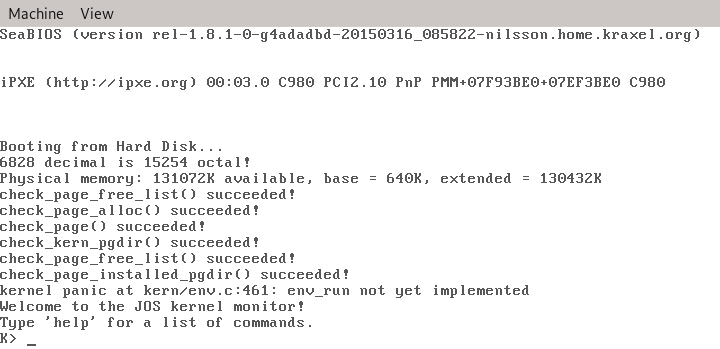
\includegraphics[width=0.8\linewidth]{lab2/exercise1_1.png}
        \caption{重新编译后运行qemu的输出}
        \label{fig:lab2/exercise1_1}
    \end{figure}
    \FloatBarrier
\end{exerciseSolution}

\section{Virtual Memory}
\exercise{2}{
    \par 阅读\textit{Intel 80386 Reference Manual}\footnote{\url{https://pdos.csail.mit.edu/6.828/2017/readings/i386/toc.htm}}的第5章和第6章,并仔细阅读有关分页转换以及基于分页的保护。
}
\begin{exerciseSolution}{2}
    \par 对于分页转换而言,需要注意的是线性地址的格式、页表的格式以及线性地址如何转换为物理地址。线性地址的31\textasciitilde 22bit为页目录地址,21\textasciitilde 12为页地址,而11\textasciitilde 0位为偏移量。线性地址到物理地址的转换过程如图\ref{fig:lab2/exercise2_1}所示。
    \begin{figure}[htb]
        \centering
        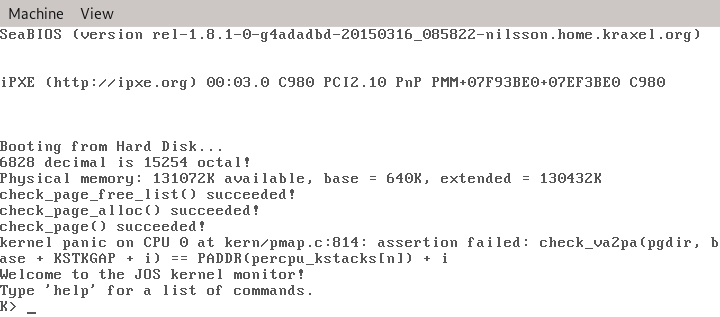
\includegraphics[width=0.7\linewidth]{lab2/exercise2_1.png}
        \caption{线性地址到物理地址的转换}
        \label{fig:lab2/exercise2_1}
    \end{figure}
    \par 而对于每一个页表项,其不仅包含物理页的地址,还包含一系列的表示位用于表示页的属性,如权限、使用标志等。基于分页的保护就是建立在这种页表项的基础之上的。基于分页的保护参数包括2个标志位,一个是页表项中的U/S位,当其为0时表示监督模式,此时这个分页用于操作系统以及系统软件,当其为1时表示用户模式,为用户态软件提供服务。另一个标志位则是R/W位,当其为0时表示只读模式,为1时则表示读写模式。
\end{exerciseSolution}

\subsection{Virtual, Linear, and Physical Addresses}
\label{sub:virtual_linear_and_physical_addresses}

\par 在x86系统中,一个虚拟地址由两部分组成:段选择器和段内偏移。线性地址值得是通过段地址转换机构把虚拟地址进行转换之后得到的地址,而物理地址则是分页地址转换机构将线性地址转换之后得到的真实内存地址。
\par C语言中的指针是虚拟地址中的段内偏移部分。boot/boot.S中的的全局描述符表将所有段的基址设置为0,上限设置为0xffffffff,因而关闭了分段管理的功能。此时虚拟地址中段选择器字段的内容失去了意义,因为线性地址的值总是等于虚拟地址中段内偏移的值。lab1 中part3引入了一个简单的页表,这个页表只映射了4MB的空间。在jOS中需要将这种映射扩展到256MB的空间上。

\exercise{3}{
    \par Gdb只能够通过虚拟地址访问qemu的内存,但如果能够访问到实际内存地址将会是十分有用的。在运行qemu的终端中按下Ctrl-a c即可进入qemu的监视器
    \par 在qemu监视器中使用xp命令以及gdb中的x命令来查看虚拟地址和对应物理地址的内存内容。对于6.828 patch版本的qemu而言,info pg能够显示页表的内容,而info mem能够显示所有已经被页表映射的虚拟地址的空间以及它们的访问优先级。
}
\begin{exerciseSolution}{3}
    \par 编译并运行qemu,在进入内核之后,在GDB中使用x命令检查0xf0100000处的部分内容,并使用qemu的xp命令检查0x00100000处的部分内容,其结果如图\ref{fig:lab2/exercise3_1}所示。
    \begin{figure}[htb]
        \centering
        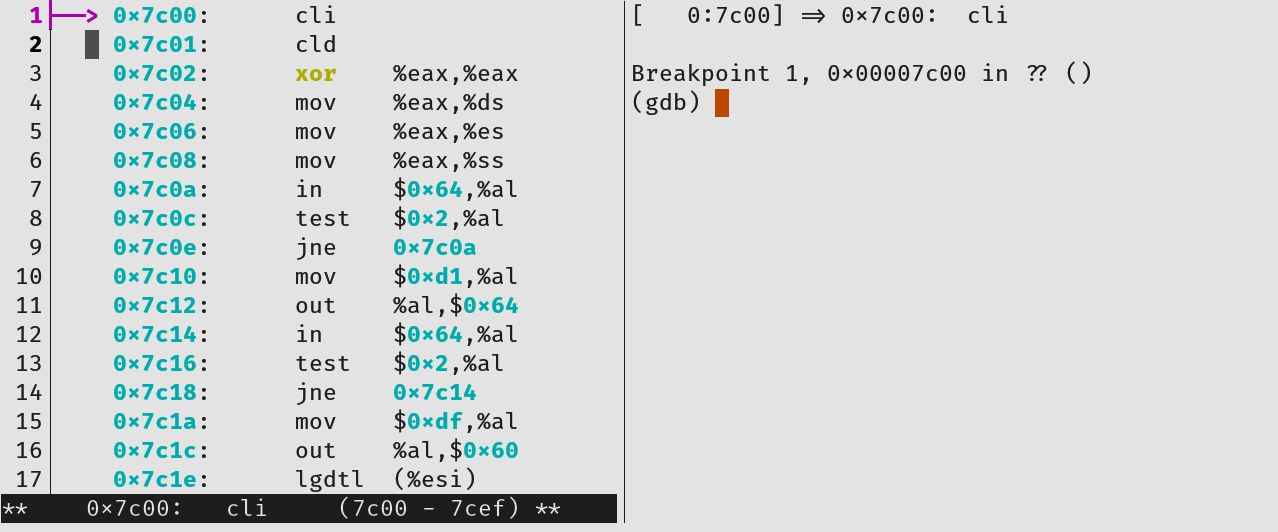
\includegraphics[width=0.95\linewidth]{lab2/exercise3_1.png}
        \caption{qemu以及gdb对于映射地址内容的显示}
        \label{fig:lab2/exercise3_1}
    \end{figure}
    \par 从图中可以看出,映射后的虚拟地址的内容和物理地址的内容是一致的。在qemu中输入info pg以及info mem后其输出如图\ref{fig:lab2/exercise3_2}所示。从图中可以看出,qmeu打印出了页表的内容以及映射的虚拟地址空间。
    \begin{figure}[htb]
        \centering
        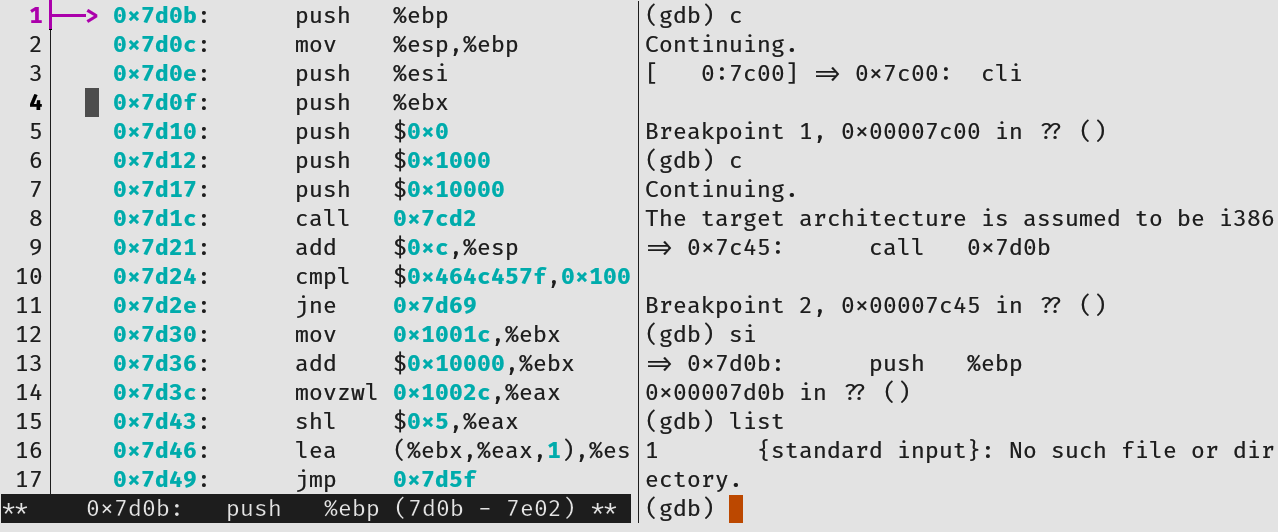
\includegraphics[width=0.6\linewidth]{lab2/exercise3_2.png}
        \caption{qemu中info pg以及info mem的输出}
        \label{fig:lab2/exercise3_2}
    \end{figure}
\end{exerciseSolution}

\par 进入保护模式之后,就不能够直接使用物理地址和线性地址了,所有代码中的地址都是虚拟地址的形式,并被MMU转换。jOS内核需要同时操作虚拟地址和物理地址但不对其解引用。为了帮助记录代码,jos中有两个类型的指针:unitptr\_t表示虚拟地址,而physaddr\_t表示物理地址。实际上,它们都是32位整型值(uint32\_t)。正因为如此编译器不会阻止将一个类型赋值给另一个类型,但是会阻止对这些值的解引用。要对其解引用,需要首先将其强制转换为一个指针类型。

\begin{questionEnv}
    \begin{enumerate}
        \item 假设以下jOS内核代码是正确的,那么x应该是unitptr\_t类型还是physaddr\_t类型?
            \inputCodeSetLanguage{c}
            \begin{lstlisting}
mystery_t x;
char* value = return_a_pointer();
*value = 10;
x = (mystery_t) value;
            \end{lstlisting}
    \end{enumerate}
\end{questionEnv}
\begin{answer}
    \begin{enumerate}
        \item 由于使用了*操作符进行了解引用,因此变量x应该为虚拟地址,是uintptr\_t类型。
    \end{enumerate}
\end{answer}

\subsection{Reference counting}
\label{sub:reference_counting}

\par 在之后的实验中将会遇到多个不同的虚拟地址被同时映射到相同的物理页面上的情况。在这种情况下我们需要记录每一个物理页面上存在多少不同的虚拟地址来引用它。这个值存放在PageInfo的pp\_ref中。当这个值变为0时物理页才可以被释放。通常情况下任意一个物理页p的pp\_ref的值等于它所在的所有页表中被虚拟地址UTOP下方的虚拟页映射的次数。

\subsection{Page Table Management}
\label{sub:page_table_management}
\par 这一部分需要创建一个页表管理程序,包括插入和删除线性地址到物理地址的映射,以及页表的创建等。

\exercise{4}{
    \par 完成kern/pmap.c中以下几个函数的实现。
    \begin{itemize}
        \item pgdir\_walk()
        \item boot\_map\_region()
        \item page\_lookup()
        \item page\_remove()
        \item page\_insert()
    \end{itemize}
    \par mem\_init中调用的check\_page可以用于检查这些函数的实现是否正确。
}
\begin{exerciseSolution}{4}
    \par 首先实现pgdir\_walk。根据注释,可以得知该函数所需要实现的功能为:给定一个页表目录指针pgdir,该函数应该返回线性地址va对应的页表项的指针。此时可能这个页不存在,当这个页不存在时如果create==true则分配新的页,否则返回NULL,也就是说实现函数时需要注意页目录项对应的页表是否存在于内存中。最终,函数的实现如下:
    \inputCodeSetLanguage{c}
    \begin{lstlisting}
pte_t *pgdir_walk(pde_t *pgdir, const void *va, int create) {
    pde_t *pgdir_entry = pgdir + PDX(va);
    if (!(*pgdir_entry & PTE_P)) {
        if (!create)
            return NULL;
        else {
            struct PageInfo *new_page = page_alloc(1);
            if (!new_page)
                return NULL;
            *pgdir_entry = (page2pa(new_page) | PTE_P | PTE_W | PTE_U);
            ++new_page->pp_ref;
        }
    }
    return (pte_t *)(KADDR(PTE_ADDR(*pgdir_entry))) + PTX(va);
}
    \end{lstlisting}

    \par 接下来是boot\_map\_region函数。这个函数要求将虚拟空间$[va, va+size)$映射到物理空间$[pa, pa+size)$的这种映射关系加入到pgdir中,其中size是PGSIZE的整数倍大小。此函数主要是为了设置UTOP之上的静态映射地址范围。最终,函数的实现如下,函数中,每一轮循环将一个物理页和虚拟也的映射关系加入到页表中,直到将size个字节分配完。
    \begin{lstlisting}
static void boot_map_region(pde_t *pgdir, uintptr_t va,
        size_t size, physaddr_t pa, int perm) {
    int offset;
    pte_t *pgtable_entry;
    for (offset = 0; offset < size; offset += PGSIZE, va += PGSIZE, pa += PGSIZE) {
        pgtable_entry = pgdir_walk(pgdir, (void *)va, 1);
        *pgtable_entry = (pa | perm | PTE_P);
    }
}
    \end{lstlisting}

    \par 对于page\_lookup函数而言,它返回va所映射的物理页的PageInfo指针,且若page\_store不为0则将物理页的页表地址存入pte\_store中,如果va没有被映射则返回NULL。其实现如下:
    \begin{lstlisting}
struct PageInfo *page_lookup(pde_t *pgdir, void *va, pte_t **pte_store) {
    pte_t *pgtable_entry = pgdir_walk(pgdir, va, 0);
    if (!pgtable_entry || !(*pgtable_entry & PTE_P))
        return NULL;
    if (pte_store)
        *pte_store = pgtable_entry;
    return pa2page(PTE_ADDR(*pgtable_entry));
}
    \end{lstlisting}

    \par 下面是page\_remove函数,其作用是将虚拟地址va的映射关系删除。其中,pp\_ref的值要减1,且如果pp\_ref减为0则需要将这个页回收,最后,这个页的页表项需要被置为0,且如果移走了这个页,TLB需要被无效化。最终的page\_remove实现如下:
    \begin{lstlisting}
void page_remove(pde_t *pgdir, void *va) {
    pte_t *pgtable_entry;
    struct PageInfo *page = page_lookup(pgdir, va, &pgtable_entry);
    if (!page)
        return;
    page_decref(page);
    tlb_invalidate(pgdir, va);
    *pgtable_entry = 0;
}
    \end{lstlisting}

    \par 最后,是对于page\_insert的实现。其功能与page\_remove相对,也就是将映射到虚拟内存中的va映射到物理内存页pp上。如果va已经映射,则应该使用page\_remove将其移除。并且页表应该按需分配并插入到pgdir中,且pp\_ref需要加一,最后的函数实现如下:
    \begin{lstlisting}
int page_insert(pde_t *pgdir, struct PageInfo *pp, void *va, int perm) {
    pte_t *pgtable_entry = pgdir_walk(pgdir, va, 1);
    if (!pgtable_entry)
        return -E_NO_MEM;
    ++pp->pp_ref;
    if ((*pgtable_entry) & PTE_P) {
        tlb_invalidate(pgdir, va);
        page_remove(pgdir, va);
    }
    *pgtable_entry = (page2pa(pp) | perm | PTE_P);
    *(pgdir + PDX(va)) |= perm;
    return 0;
}
    \end{lstlisting}

    \par 将这些函数补充完整后,重新编译并启动qemu。qemu的输出结果如图\ref{fig:lab2/exercise4_1}所示。
    \begin{figure}[htb]
        \centering
        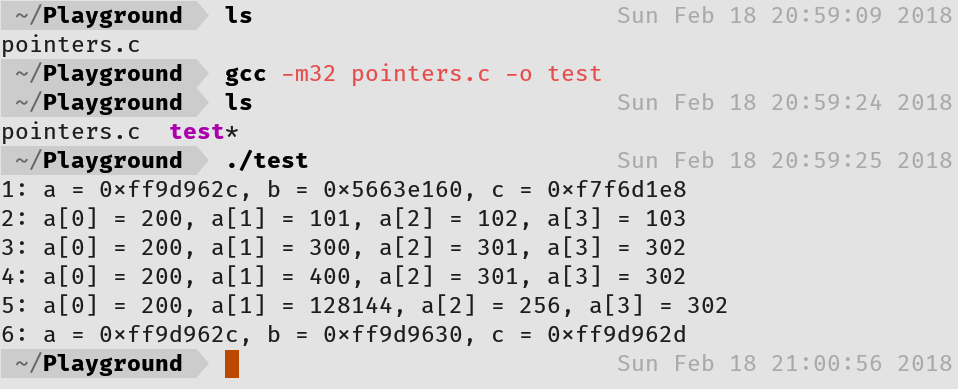
\includegraphics[width=0.7\linewidth]{lab2/exercise4_1.png}
        \caption{重新编译运行后qemu的输出}
        \label{fig:lab2/exercise4_1}
    \end{figure}
    \par 从图中可以看到,check\_page的检查已经通过,说明上述5个函数的实现基本正确,接下来的kernel panic需要在下一个实验中解决。
    \FloatBarrier
\end{exerciseSolution}

\section{Kernel Address Space}
\label{sec:kernel_address_space}
\par jOS将处理器的线性地址划分为占用低地址的用户环境和占用高地址的内核,其界限是inc/memlayout.h中的变量ULIM。jOS为内核保留了256M的地址空间,这也就是为什么在Lab 1中要给操作系统设计一个非常高的地址空间。

\subsection{Permissions and Fault Isolation}
\label{sub:permissions_and_fault_isolation}
\par 由于内核和用户进程只能访问各自的地址空间,所以我们不许在x86中使用权限位来将用户的代码限制在只能访问在用户空间可写权限位PTE\_W可以同时影响内核和用户代码。高于ULIM的内存内核可读写但用户没有权限。用户和内核在$[UTOP, ULIM)$有同样的可读不可写权限。低于UTOP的地址是用户空间。

\subsection{Initializing the Kernel Address Space}
\label{sub:initializing_the_kernel_address_space}

\par 在这一部分,需要设置UTOP之上的,给内核使用的空间。inc/memlayout.h展示了应该使用的内存布局。

\exercise{5}{
    \par 将mem\_init()内的check\_page()之后的代码补充完整。可以使用check\_kern\_pgdir()以及check\_page\_installed\_pgdir()来检查实现的代码。
}
\begin{exerciseSolution}{5}
    \par 根据mem\_init中check\_page之后的注释。首先,我们需要将pages数组映射到线性地址UPAGES上,此处使用boot\_map\_region函数进行映射,添加的代码为:
    \inputCodeSetLanguage{c}
    \begin{lstlisting}
boot_map_region(kern_pgdir, UPAGES, PTSIZE, PADDR(pages), PTE_U);
    \end{lstlisting}
    \par 然后映射物理地址到内核的栈区域,将bootstack标记的物理地址映射到内核的堆栈。但是只需要映射$[KSTACKTOP-KSTKSIZE, KSTACKTOP)$这部分区域。因此此处补充的代码为:
    \begin{lstlisting}
boot_map_region(kern_pgdir, KSTACKTOP - KSTKSIZE, KSTKSIZE, PADDR(bootstack), PTE_W);
    \end{lstlisting}

    \par 最后,映射虚拟地址$[KERNBASE, 2^{32})$到物理地址$[0, 2^{32} - KERNBASE)$,内核的权限为读写,因此补充的代码为:
    \begin{lstlisting}
boot_map_region(kern_pgdir, KERNBASE, (0xffffffff-KERNBASE), 0, PTE_W);
    \end{lstlisting}
    \par 最后,重新编译jOS并启动qemu,其输出如图\ref{fig:lab2/exercise5_1}所示。从图中可以看出,所有的测试已经通过。
    \begin{figure}[htb]
        \centering
        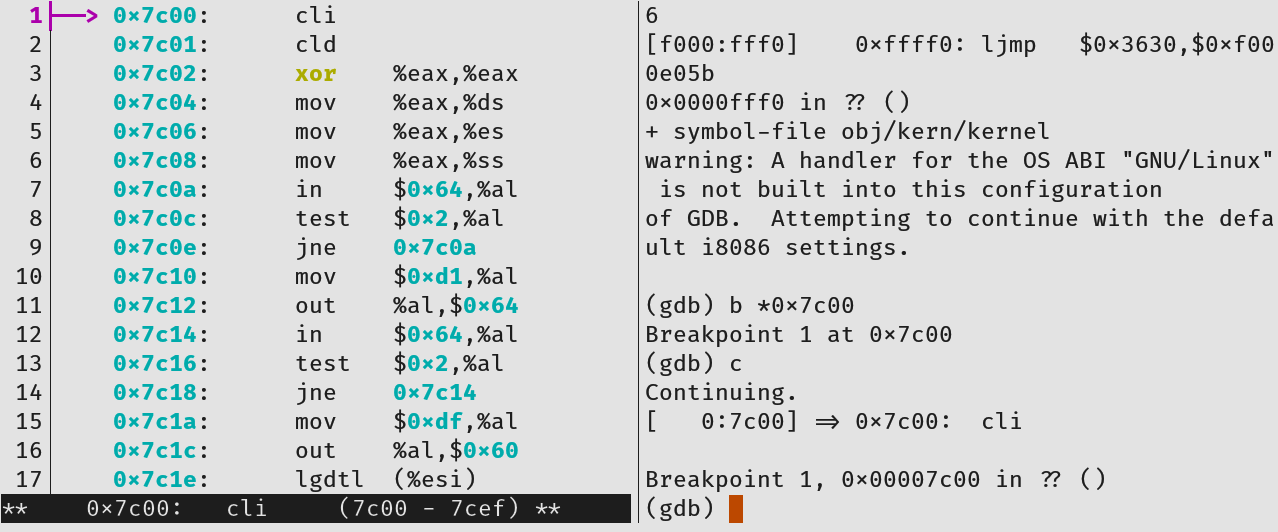
\includegraphics[width=0.8\linewidth]{lab2/exercise5_1.png}
        \caption{重新编译并启动qemu后的输出结果}
        \label{fig:lab2/exercise5_1}
    \end{figure}
    \FloatBarrier
\end{exerciseSolution}

\begin{questionEnv}
    \begin{enumerate}
        \setcounter{enumi}{1}
    \item 至此page directory被填入了哪些行?它们又被映射到了哪里?填写下面这张表。
        \begin{center}
            \begin{tabular}{c c c}
                \toprule
                Entry & Base Virtual Address & Points to (logically) \\
                \cmidrule(lr){1-3}
                1023 & ? & Page table for top 4MB of phys memory \\
                1022 & ?          & ? \\
                .    & ?          & ? \\
                .    & ?          & ? \\
                .    & ?          & ? \\
                2    & 0x00800000 & ? \\
                1    & 0x00400000 & ? \\
                0    & 0x00000000 & [see next question] \\
                \bottomrule
            \end{tabular}
        \end{center}
    \item 如果我们把kernel和user environment放在同一个地址空间中,为什么用户程序不能读写内核的内容?什么机制防保护了内核空间?
    \item 这个操作系统最大可以支持多少内存?为什么?
    \item 如果现在有最大的物理内存,那么我们需要多找额外的空间管理这些内存?这些额外的空间是怎么组成的?
    \item 回顾kern/entry.S以及kern/entrypgdir.c。在分页刚被打开时,EIP仍然是一个很低的数(1MB多一点)。在哪里EIP变得比KERNBASE高的?在刚开启分页到EIP比KERNBASE高的这段时间内,是什么让EIP保持一个很小的值但是程序继续运行的?为什么这种转换是必要的?
\end{enumerate}
\end{questionEnv}
\begin{answer}
    \begin{enumerate}
        \setcounter{enumi}{1}
    \item 通过inc/memlayout.h,可以知道page directory实际如下:
        \begin{center}
            \begin{tabular}{c c c}
                \toprule
                Entry & Base Virtual Address & Points to (logically) \\
                \cmidrule(lr){1-3}
                1023 & 0xffc00000 & Page table for top 4MB of phys memory \\
                ...  & ...        & ...           \\
                960  & 0xf0000000 & KERNBASE      \\
                959  & 0xefc00000 & Kernel Stack  \\
                957  & 0xef400000 & Page Directory\\
                956  & 0xef000000 & PageInfo array\\
                ...  & ...        & ...           \\
                0    & 0x00000000 & Empty         \\
                \bottomrule
            \end{tabular}
        \end{center}
    \item 因为用户不能访问没有PTE\_U权限的页,叶保护机制保护了内核空间。
    \item 最大可以支持4G的空间。
    \item 执行了一下代码以后EIP变得比KERNBASE高。
        \begin{lstlisting}
mov	$relocated, %eax
jmp	*%eax
        \end{lstlisting}
        \par 之所以代码能够继续执行,是因为0\textasciitilde 4MB的地址空间映射到了0\textasciitilde 4MB的物理地址(kern/entrypgdir.c)中。转换的必要性在于需要在高地址处执行代码。
\end{enumerate}
\end{answer}


